\documentclass{if-beamer}
\begin{document}
	
	\title[Campus Formoso do Araguaia]{Matemática Aplicada e noções de Educação financeira}
	\subtitle{Aula 0 }
	\author{Gilmar Gomes do Nascimento}
	\institute[IFTO]{
		Instituto Federal do Tocantins\\
		Campus Formoso do Araguaia
	}
	\date{\today}
	\logo{
		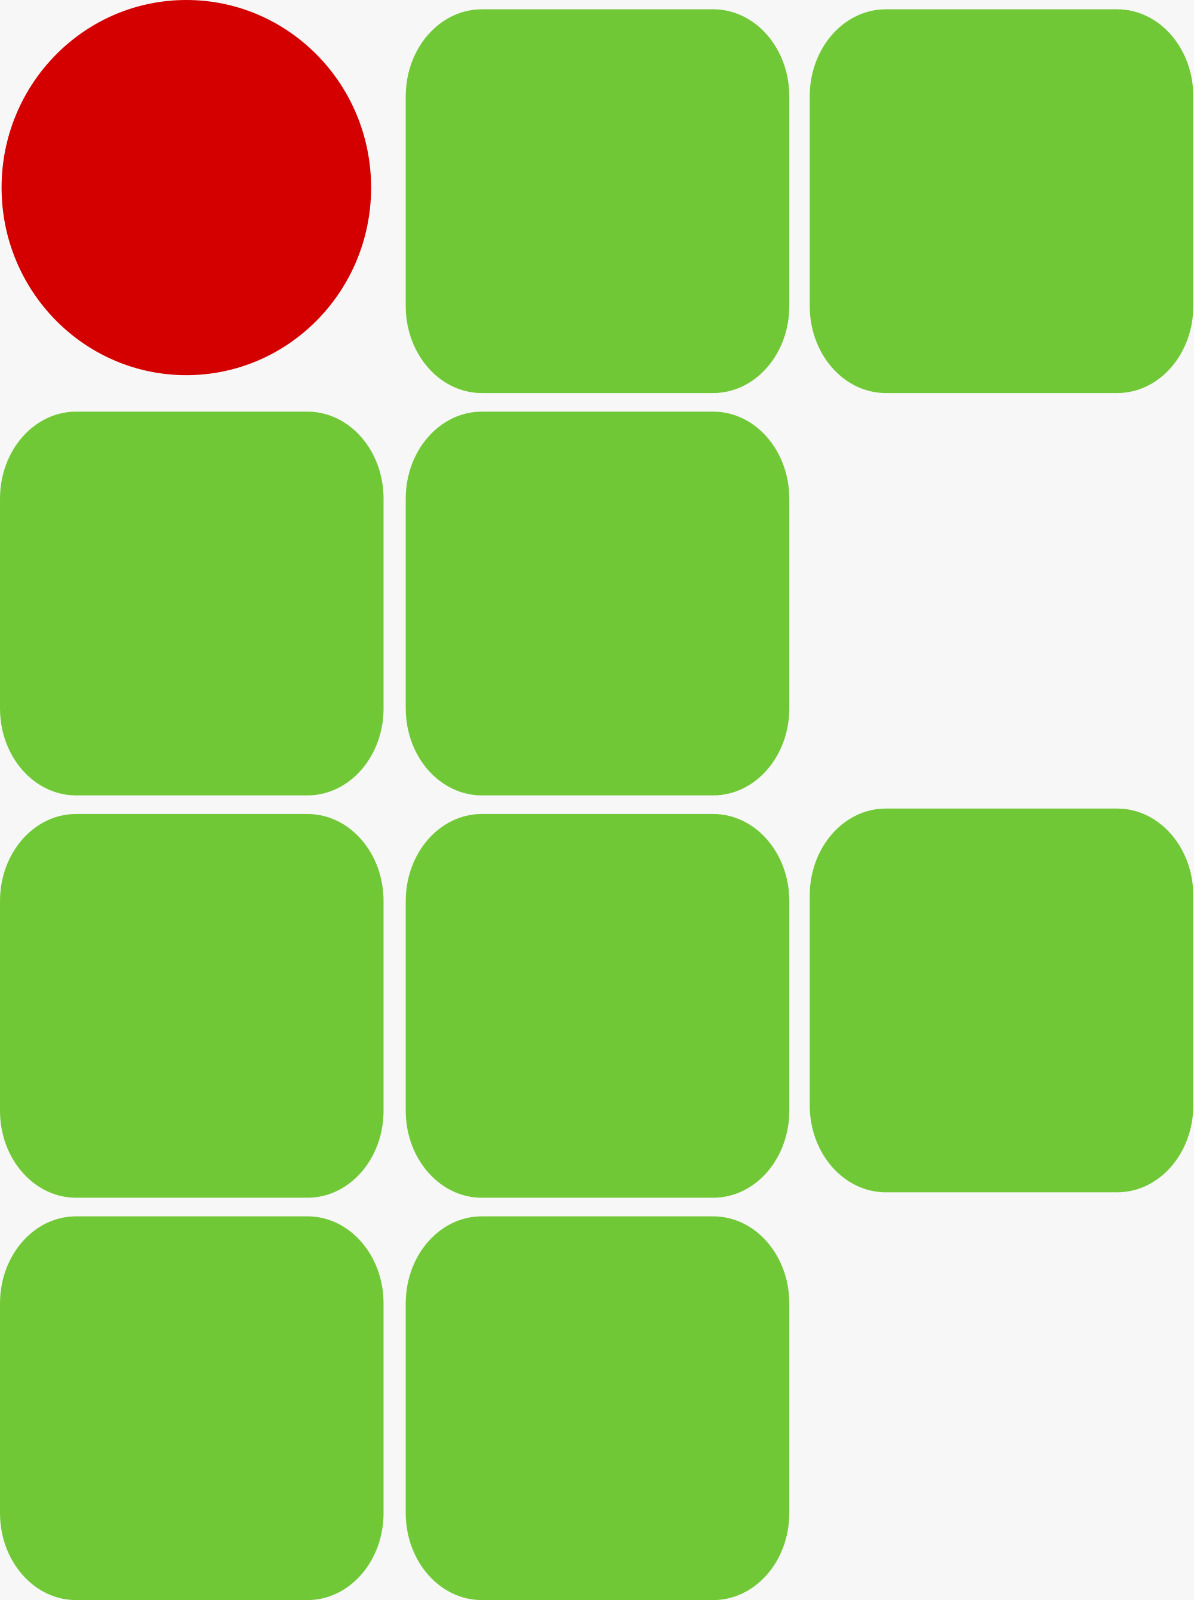
\includegraphics[scale=0.0085]{logo.jpg}
	}
	\subject{Math} % metadata
	
	\graphicspath{{figuras/}}
	%---------------------------------------------------------------------------------
	\begin{frame}
		\titlepage
	\end{frame}
	
%	\begin{frame}{Formação Acadêmica}
%	\begin{itemize}
%	\item Ciência da Computação - UFT   2009 -- 2014
%	\item Especialização Lato Senso - ESAB - 2019
%	\item Especialização Lato Senso - Focus - 2021
%	\item Mestrado em Ciência da Computação - UTFPR - 2024 - atualmente 
%	\end{itemize}
%	
%	\end{frame}
%	
%	\begin{frame}{Atuação Profissional}
%	\begin{itemize}
%	\item Instrutor de Informática  - SENAC - TO  - 2014, 2015
%	\item Professor de Informática - Colégio da Polícia Militar - TO - 2015 - 2016
%	\item Analista de Suporte -  Justiça Federal  - TO - 2017 
%	\item Professor substituto EBTT - IFTO - Campus Colinas do Tocantins - 2017 - 2019
%	\item Professor EBTT - IFAM - Campus Boca do Acre - 2021 - 2026
%	\item Professor EBTT - IFTO - Campus Formoso do Araguaia - 2026
%	\end{itemize}
%	\end{frame}
	
	
	\begin{frame}{Matemática Aplicada e Noções de Educação Financeira}
	\begin{block}{Componente Curricular}
		Matemática aplicada e Noções de Educação Financeira e 
		Inclusão Digital voltada para Exercício da Cidadania		
	\end{block}
	\begin{block}{Carga Horária}
		20 horas		
	\end{block}
	\begin{block}{Eixo tecnológico}
		Recursos Naturais		
	\end{block}
	\end{frame}

	\begin{frame}{Ementa}
		Noções de Matemática básica e financeira. Operações com números
		inteiros e racionais aplicados nos cálculos com dinheiro e 
		movimentação financeira. Introdução aos conceitos de renda, custo, lucro, desconto e juros. Introdução ao conceito de porcentagem aplicado ao cálculo de juros e desconto. Fluxo de caixa. Estoque e controle. Noções de produção e custos. Custos	fixos e variáveis. Formação de preço de venda. Inclusão digital como instrumento de promoção da equidade, ampliação do acesso à informação, à comunicação e às oportunidades, independentemente da localização geográfica ou condição socioeconômica.		
	\end{frame}

	\begin{frame}[allowframebreaks]{Educação financeira}
		\begin{quote}
			Educação financeira é o conjunto de conhecimentos, habilidades e atitudes que permitem gerenciar o dinheiro de forma consciente, planejada e estratégica, promovendo estabilidade e realização de objetivos financeiros.
		\end{quote}

	\framebreak

		\begin{quote}
			Educação financeira envolve aprender a controlar gastos, poupar, investir e planejar o futuro financeiro, transformando conhecimento em práticas que melhoram a gestão do dinheiro e evitam endividamento excessivo
		\end{quote}

		\framebreak

		Não se trata apenas de economizar, mas de desenvolver hábitos financeiros saudáveis, compreender produtos financeiros, juros, crédito e tomar decisões informadas para alcançar metas de curto, médio e longo prazo.

		\framebreak
		A educação financeira impacta diretamente a qualidade de vida e o bem-estar, reduzindo estresse e ansiedade causados 	por má gestão financeira. Ela permite criar reservas de emergência, planejar 	a aposentadoria e realizar sonhos como viagens, compra de imóveis ou investimentos estratégicos.
		
		\framebreak
		Além disso, contribui para a disciplina financeira, tornando o dinheiro mais produtivo e permitindo decisões conscientes sobre consumo e investimentos. 
	\end{frame}

	
	\begin{frame}{Matemática Financeira}
		\begin{itemize}
			\item Foco técnico: Usa números, porcentagens e fórmulas.
			\item Objetivo: Calcular juros simples e compostos, descontos, parcelas e o retorno de investimentos.
			\item Papel: É a ferramenta que mostra o custo exato de um empréstimo ou o rendimento de uma aplicação.
		\end{itemize}
	\end{frame}
	
	\begin{frame}{Educação Financeira}
		\begin{itemize}
			\item Foco comportamental: Trabalha hábitos, atitudes e a relação da pessoa com o dinheiro.
			\item Objetivo: Ensinar a diferenciar desejos de necessidades, evitar dívidas e planejar o futuro.				\item Papel: É a base que orienta como e por que gastar, poupar ou investir de forma consciente.
		\end{itemize}
	\end{frame}
	
	\begin{frame}{Diferenças entre Matemática Financeira e Educação Financeira}
		A principal diferença é que a \textbf{matemática financeira} foca nos cálculos e fórmulas para medir o dinheiro ao longo do tempo, enquanto a \textbf{educação financeira} lida com comportamentos, escolhas e planejamento de vida.		
	\end{frame}

	\begin{frame}[allowframebreaks]{Comportamento}
		\begin{quote}
			O comportamento financeiro estuda como emoções, crenças e hábitos influenciam nossas decisões econômicas, impactando desde gastos cotidianos até investimentos complexos.
		\end{quote}
		
		\framebreak

		O comportamento financeiro é um campo que analisa a interação entre psicologia e economia, mostrando que nossas decisões sobre dinheiro nem sempre são racionais. Fatores emocionais como:

		 \begin{itemize}
			\item Ansiedade
			\item Impulso
			\item Acúmulo
		 \end{itemize}

	\framebreak
	
		\begin{block}{Bem-estar financeiro}
			Podem levar a escolhas pouco estratégicas, afetando diretamente o bem-estar financeiro. Ele abrange desde decisões simples, como poupar ou gastar, 	até decisões complexas, como investir ou contrair dívidas.
		\end{block}
	\end{frame}

	\begin{frame}{Gestão de dinheiro}
		Compreender o comportamento financeiro é essencial para uma gestão de dinheiro mais inteligente e estratégica, permitindo reconhecer padrões prejudiciais, minimizar riscos e melhorar a tomada de decisão em todas as áreas da vida econômica. Ele oferece uma perspectiva que vai além da lógica pura, considerando a complexidade da mente humana e suas influências sobre o dinheiro.
	\end{frame}
	
	\begin{frame}{Econômico ou mão de vaca?}
		\begin{figure}
			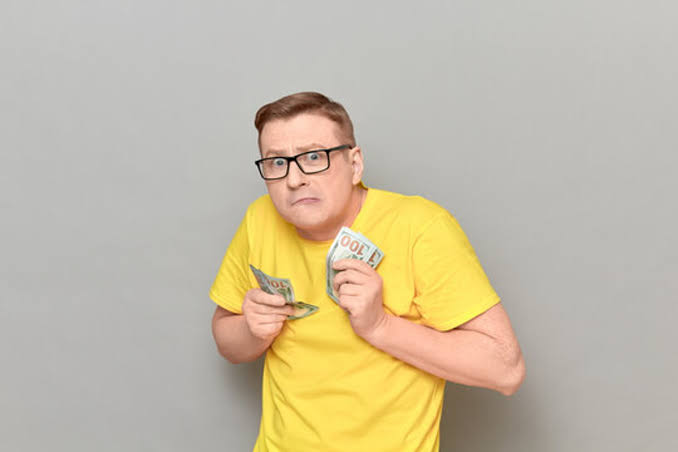
\includegraphics[scale=0.3]{mao-de-vaca}
		\end{figure}
		``Mão de vaca" ~ é uma expressão usada para descrever uma pessoa avarenta, muito apegada ao dinheiro e que evita gastar, sendo sinônimo de sovina, pão-duro ou mesquinho.
	\end{frame}
	
	\begin{frame}{Economia}
		\begin{figure}
			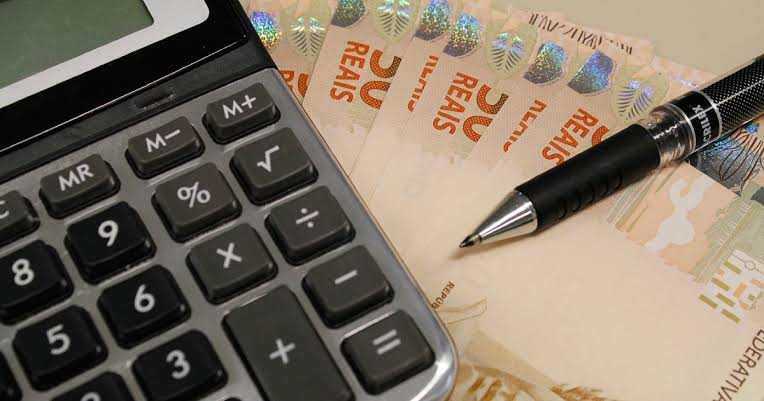
\includegraphics[scale=0.39]{economia}
		\end{figure}
	\end{frame}
	
	\begin{frame}[allowframebreaks]{Economia Solidária}
		Economia solidária é definida como o ``conjunto de atividades econômicas -- de produção, distribuição, consumo, poupança e crédito -- organizadas sob a forma de autogestão."
	
	\framebreak
	
	Compreende uma variedade de práticas econômicas e sociais organizadas sob a forma de cooperativas, associações, clubes de troca, empresas autogestionárias, redes de cooperação, entre outras, que realizam atividades de produção de bens, prestação de serviços, finanças solidárias, trocas, comércio justo e consumo 		solidário.
	 
	\framebreak
	 Trata-se de uma forma de organização da produção, consumo e distribuição de riqueza centrada na valorização do ser humano e não do capital, caracterizada pela igualdade.

	\framebreak
	
	``A economia solidária é uma alternativa inovadora na geração de trabalho e na inclusão social, na forma de uma corrente do bem que integra quem produz, quem vende, quem troca e quem compra. Seus princípios são autogestão, democracia, solidariedade, cooperação, respeito à natureza, comércio justo e consumo 				solidário."
	
	\framebreak
	
	A economia solidária preconiza o entendimento do trabalho como um meio de emancipação humana dentro de um processo de democratização econômica, criando uma alternativa à dimensão alienante e assalariada das relações de trabalho capitalistas.
	
	\framebreak
	
	Além disso, a economia solidária possui uma finalidade multidimensional, isto é, envolve a dimensão social, econômica, política, ecológica e cultural. Isto porque, além da visão econômica de geração de trabalho e renda, as experiências de economia solidária se projetam no espaço público, tendo como perspectiva a 	construção de um ambiente socialmente justo e sustentável. 
	
	\framebreak
	
	Vale ressaltar que a economia solidária não se confunde com o chamado ``terceiro setor", que substitui o Estado nas suas obrigações legais e inibe a emancipação de trabalhadores, enquanto sujeitos protagonistas de direitos. A economia solidária reafirma, assim, a emergência de atores sociais, ou seja, a 		emancipação de trabalhadores como sujeitos históricos.

	\end{frame}
	
%	\begin{frame}{Em outras palavras}
%		\begin{figure}
%			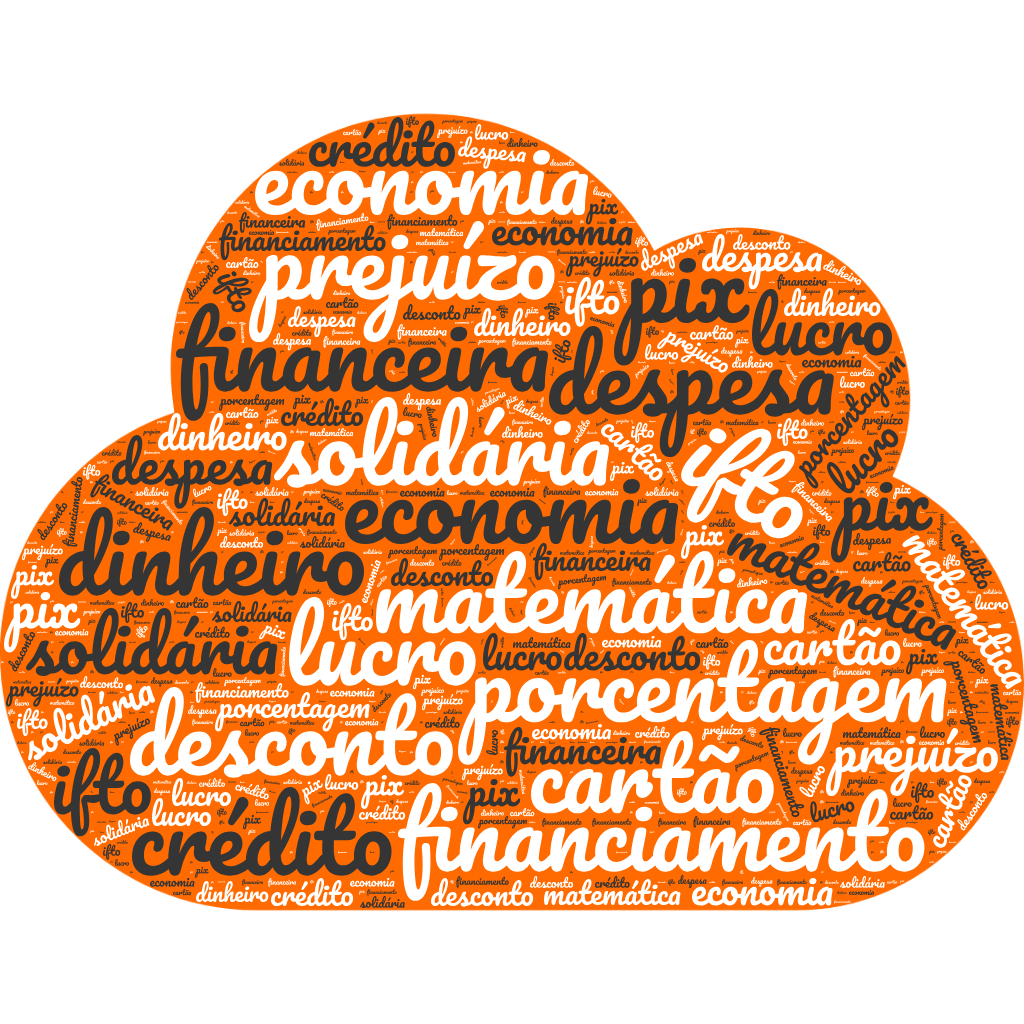
\includegraphics[scale=0.2]{cloud-words.png}
%		\end{figure}
%	\end{frame}
	
	\begin{frame}{Vídeos extras e comentados na aula}
		\url{https://www.youtube.com/watch?v=o3WSiFv4tGA} \\
		\url{https://www.youtube.com/watch?v=KiohYOY60Ug}
	
		\begin{figure}
			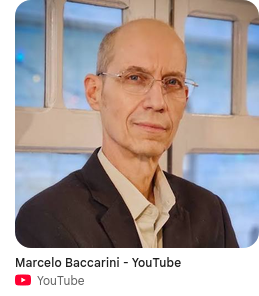
\includegraphics[scale=0.5]{marcelo-baccarini.png}
		\end{figure}
	\end{frame}
	

\begin{frame}[allowframebreaks]{Referências Bibliográficas}
    \begin{thebibliography}{9}
        \bibitem{pianezzer2025educaccao}
        Pianezzer, G. A. e Silva Junior, E. (2025). Educação e Matemática Financeira: diferenças, intersecções e implicações no contexto educacional brasileiro. \textit{Caderno Intersaberes}, 14(52):263--271.

        \bibitem{Santander}
        O que é educação financeira, quais os seus pilares e por que é importante? \textit{Santander Blog}. \url{https://www.santander.com.br/blog/o-que-e-educacao-financeira}. Acessado em: 31 de agosto de 2026.

        \bibitem{Conceito.de}
        Educação financeira. \textit{Conceito.de}. \url{https://conceito.de/educacao-financeira}. Acessado em: 31 de agosto de 2026.

        \bibitem{Caixa}
        Educação Financeira. \textit{Caixa}. \url{https://www.caixa.gov.br/educacao-financeira/Paginas/default.aspx}. Acessado em: 31 de agosto de 2026.
%
%\framebreak
%        \bibitem{Azul2022-lg}
%        Azul, E. C. (2022). Preço de custo vs preço de venda: como calcular e definir o preço ideal. \textit{Blog da Conta Azul}. \url{https://contaazul.com/blog/preco-de-custo-e-preco-de-venda/}. Acessado em: 31 de agosto de 2026.
%
        \bibitem{Revista Ecotur}
        Diferença entre educação financeira e matemática financeira. \textit{Revistaecotour.news}. \url{https://www.revistaecotour.news/2025/06/diferenca-entre-educacao-financeira-de.html}. Acessado em: 31 de agosto de 2026.

%        \bibitem{wikipidia2025}
%        Wikipédia. (2025). Economia solidária. \url{https://pt.wikipedia.org/w/index.php?title=Economia_solid%C3%A1ria&oldid=70924717}. Acessado em: 26 de setembro de 2025.
%
        \bibitem{governo2026}
        Economia Solidária. \textit{Ministério do Trabalho e Emprego}. \url{https://www.gov.br/trabalho-e-emprego/pt-br/assuntos/economia-solidaria}. Acessado em: 31 de agosto de 2026.

%        \bibitem{observatorio2026}
%        O que é a Economia Solidária? \textit{Observatório Nacional da Economia Solidária e do Cooperativismo}. \url{https://ecosol.dieese.org.br/o-que-e-a-economia-solidaria/}. Acessado em: 31 de agosto de 2026.
%
    \end{thebibliography}
\end{frame}
\end{document}
